\documentclass[a4paper,12pt]{article}

\usepackage[T2A]{fontenc}
\usepackage[utf8]{inputenc}

\usepackage[english,russian]{babel}
\usepackage{amsmath,amsfonts,amssymb,amsthm,mathtools}
\usepackage{graphicx}

\author{Happy Helio}
\title{Общие принципы и математика в \LaTeX{}}
\date{\today}

\begin{document}
\maketitle
\newpage

\section{Обычный текст}

Наша первая строка \\ 
Важное можо выделить \textbf{жирным} \\
\textit{Строка, написанная курсивом} \\
\underline{Подчеркнутный текст}
\fbox{текст в рамке} \\
Дефис -- не тире \\
Дефис -  не тире \\
<<Кавычки>>

\section{Мир формул}

Наша первая формула $100+100=200$, ага.
\[100+100=200\] %формула по середине

\begin{equation}\label{pifagor}
a^2+b^2=c^2
\end{equation}

Теорема Пифагора \eqref{pifagor} изучается в 8-ом классе. 
Она упоминается на странице \pageref{pifagor}

\subsection{Дроби} 

% Для того чтобы убрать нумерацию разделов, подразделов
% необходимо поставить *
% Пример:  \subsection*{Рациональные дроби}

$\frac{1}{3}+\frac{1}{3}=\frac{2}{3}$ Вот вам и дроби. Выглядит не очень.

\[\frac{1}{3}+\frac{1}{3}=\frac{2}{3}\]
А так намного лучше.

\subsection{Скобки}

\[ (2+3)\times 5=25\]

\[ (\frac{4}{2}+3)\times 5=25 \]

\[ \left[\frac{4}{2}+3\right]\times 5 =25 \]

\[ \left(\frac{4}{2}+3\right)\times 5 =25 \]

\[ \left\{\frac{4}{2}+3\right\}\times 5 =25 \]


\subsection{Индексы}

Грузы массой $m_1$, $m_{12}$ \\
Тоже самое:

\[ m_1, m_{12} \]

\subsection{Стандартные формулы}

\[ \sin x=0 \]
\[ \arctan x=\sqrt[5]{3} \]
\[ \log_{x-1}{(x^2-4x+5)} \geqslant 2\]
\[ \lg_{x-1}{(x^2-4x+5)} \geqslant 2\]
\[ \ln_{x-1}{(x^2-4x+5)} \geqslant 2\]

\subsection{Не очень стандартные формулы}

\[\sum_{i=1}^{n}a_i \times b_i \]

\[I = \int r^2dm \]

\[I = \int_{0}^{1} r^2dm \]

\[I = \int\limits_{0}^{1} r^2dm \]

\subsection{Символы}

\[2\times 2\neq 5 \]

\[x \cap y \]


\newpage

\begin{center}
Вторая часть
\end{center}



\begin{flushright}
По умолчанию суффикс для запасных копий «~», если только не установлена
переменная окружения или не задан параметр.
\end{flushright}


\begin{enumerate}

\item Общие вопросы
\item Работа с текстом 
\item Математика

\begin{itemize}
\item Дроби;
\item Скобки;
\item Многое другое;
\end{itemize}

\end{enumerate}

\subsection{Диакритические знаки}

\[ \dot{x}=0,\]
\[ \tilde{a}=\bar{b}, \]
\[ \tilde{a}=\overline{bcde}, \]
\[ \overrightarrow{a} (0,3,4), \]
\[ \underbrace{1+2+3+\dots+n}_{n}=N, \]
\[ \overbrace{1+2+3+\dots+n}^{n}=N, \]
\[ (x-1)(x+1)>0 \stackrel{x>0}{\Longleftrightarrow} x-1>0, \]

\subsection{Буквы других алфавитов и математические шрифты}
\[ \sin \alpha =0 \]
\[ \omega =  \frac{2\pi}{T} \]
\[ x \in \mathbb{R} \]
\[ m_{\text{груза}}= 15~\text{кг} \]


\subsection{Матрицы}

\[ \begin{pmatrix}

a_{11} & a_{12} & a_{13} \\
a_{21} & a_{22} & a_{23} \\
a_{31} & a_{32} & a_{33} \\

\end{pmatrix} \]


\[ \begin{bmatrix}

a_{11} & a_{12} & a_{13} \\
a_{21} & a_{22} & a_{23} \\
a_{31} & a_{32} & a_{33} \\

\end{bmatrix} \]


\[ \begin{vmatrix}

a_{11} & a_{12} & a_{13} \\
a_{21} & a_{22} & a_{23} \\
a_{31} & a_{32} & a_{33} \\

\end{vmatrix} \]


\[ \begin{Vmatrix}

a_{11} & a_{12} & a_{13} \\
a_{21} & a_{22} & a_{23} \\
a_{31} & a_{32} & a_{33} \\

\end{Vmatrix} \]


\section{Группировка формул}


% Выравнивание по знаку равно
\begin{equation}
\begin{aligned}
2 \times a &= 4,\\
-3 \times b &= 6, \\
-10 \times c &= 1110.
\end{aligned}
\end{equation}


\[ \left\{
\begin{aligned}
2 \times a &= 4,\\
-3 \times b &= 6, \\
-10 \times c &= 1110.
\end{aligned} \right. 
\]

\[ \left[
\begin{aligned}
2 \times a &= 4,\\
-3 \times b &= 6, \\
-10 \times c &= 1110.
\end{aligned} \right.
\]


\[ \left.
\begin{aligned}
2 \times a &= 4,\\
-3 \times b &= 6, \\
-10 \times c &= 1110.
\end{aligned} \right\} \Rightarrow -6ab=24
\]



\section{Работа с картинками и таблицами}

% Растровые 
% Векторные

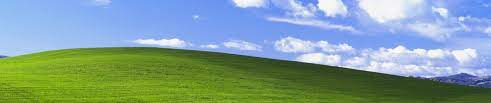
\includegraphics[scale=0.5]{landscape.jpeg}
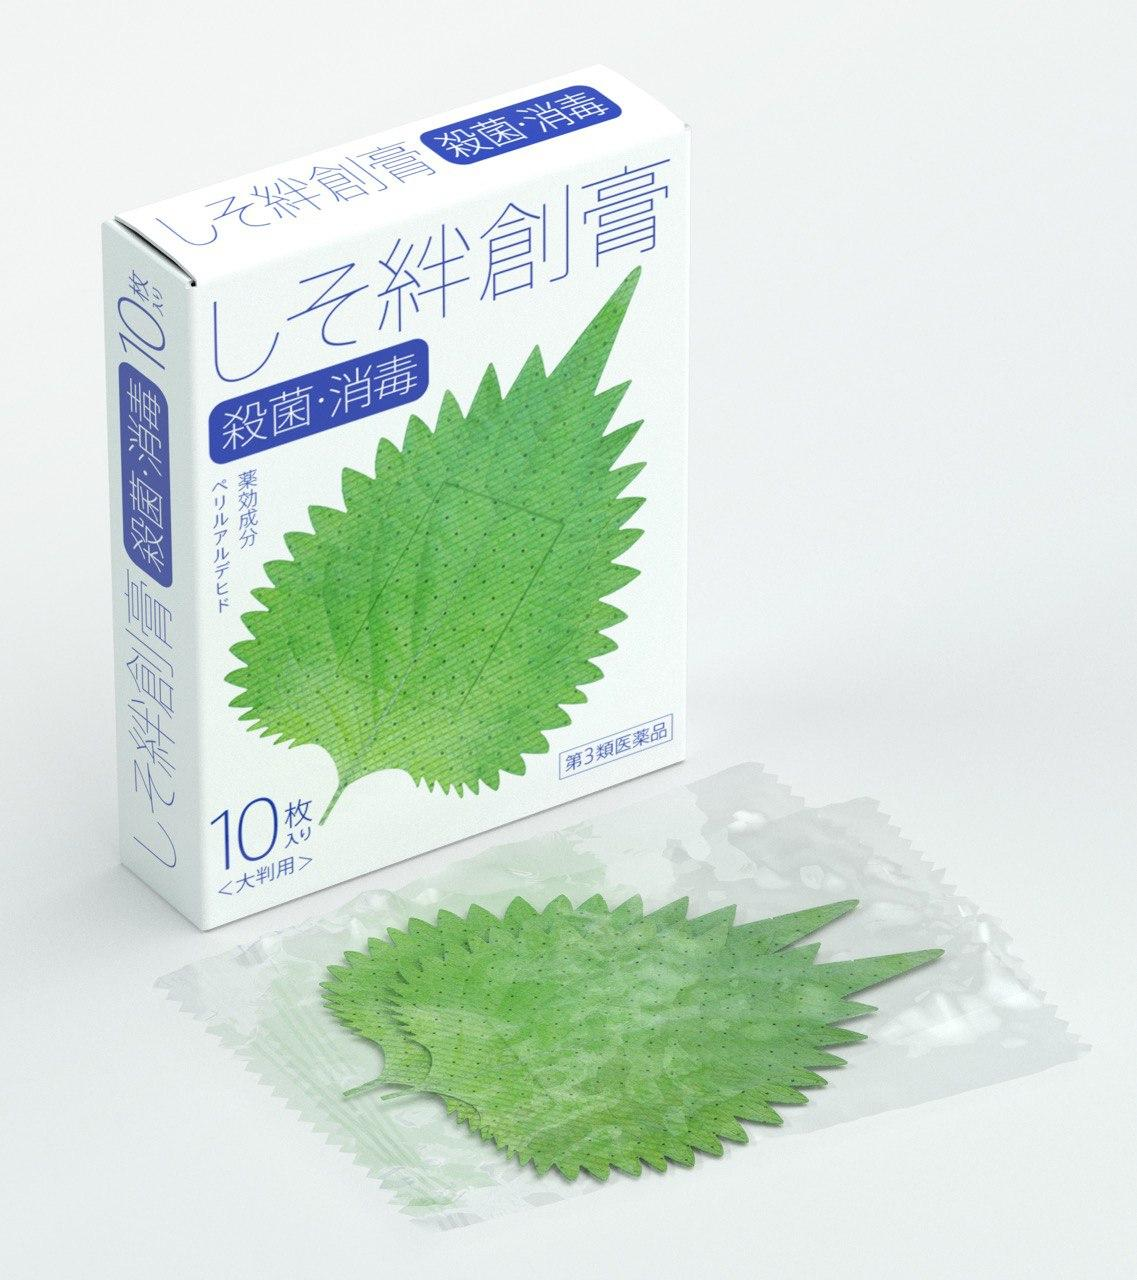
\includegraphics[width=2cm]{photo.jpg}


\begin{figure}

\begin{center}
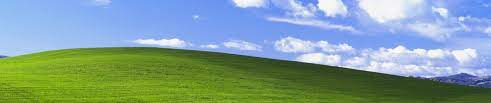
\includegraphics[scale=0.8]{landscape.jpeg}
\end{center}
\caption{Подпись 1} \label{landscape}

\end{figure}

Картинка предствлена: \ref{landscape}

	
\section{Таблицы}

\begin{right}

\begin{tabular}{|c|c|r|p{5cm}r|}
\hline
\multicolumn{3}{|c|}{Погрешности} & Подробнейший комментрарий
\hline
Систематическая & Случайная & Итог & \\
\hline
0.04 & 0.03 & 0.05 & \\
\hline
\end{tabular}

\end{right}

\end{document}




